\documentclass[UTF8,12pt]{ctexart}
\usepackage[a4paper,margin=1.5cm]{geometry}
\usepackage{graphicx}
\usepackage{float}
\usepackage{caption}
\setlength{\parindent}{0pt}
\captionsetup{font=small,labelformat=empty}
\begin{document}
\section*{高一数学专题题目归档：平面向量}
来源：\verb|documents/高一|，按 OCR 关键词筛选后裁剪原题图。共 23 题。

\subsection*{1. 原卷第 6 题}
\textbf{来源}：【期末】上海师范大学附属中学2024-2025学年第二学期高一数学期末试卷

\begin{figure}[H]
\centering
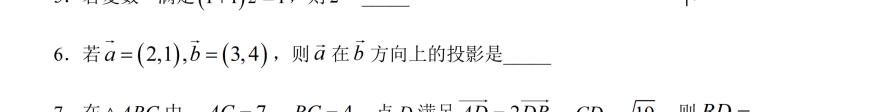
\includegraphics[width=0.96\linewidth]{crops/01-yziAF5kAbRtk3MMO-002-q06.png}
\caption{原图：\detokenize{documents/高一/01-yziAF5kAbRtk3MMO/002.png}}
\end{figure}
\vspace{0.4em}
\subsection*{2. 原卷第 7 题}
\textbf{来源}：【期末】上海师范大学附属中学2024-2025学年第二学期高一数学期末试卷

\begin{figure}[H]
\centering
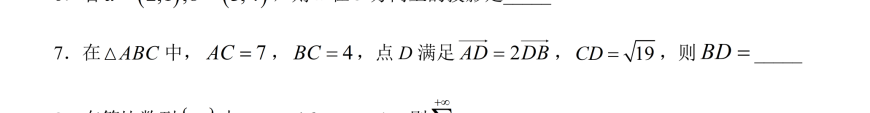
\includegraphics[width=0.96\linewidth]{crops/01-yziAF5kAbRtk3MMO-002-q07.png}
\caption{原图：\detokenize{documents/高一/01-yziAF5kAbRtk3MMO/002.png}}
\end{figure}
\vspace{0.4em}
\subsection*{3. 原卷第 15 题}
\textbf{来源}：【期末】上海师范大学附属中学2024-2025学年第二学期高一数学期末试卷

\begin{figure}[H]
\centering
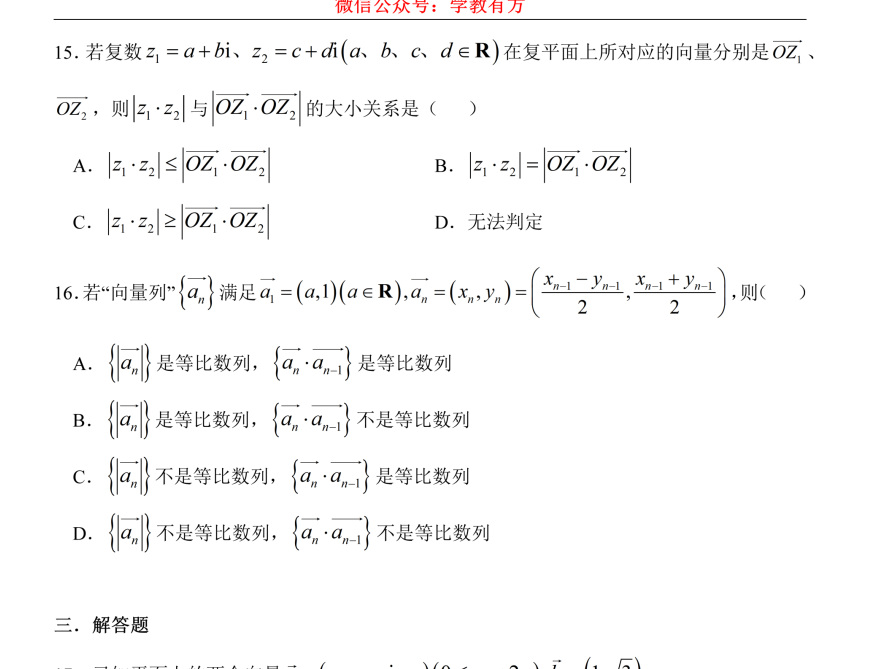
\includegraphics[width=0.96\linewidth]{crops/01-yziAF5kAbRtk3MMO-003-q15.png}
\caption{原图：\detokenize{documents/高一/01-yziAF5kAbRtk3MMO/003.png}}
\end{figure}
\vspace{0.4em}
\subsection*{4. 原卷第 17 题}
\textbf{来源}：【期末】上海师范大学附属中学2024-2025学年第二学期高一数学期末试卷

\begin{figure}[H]
\centering
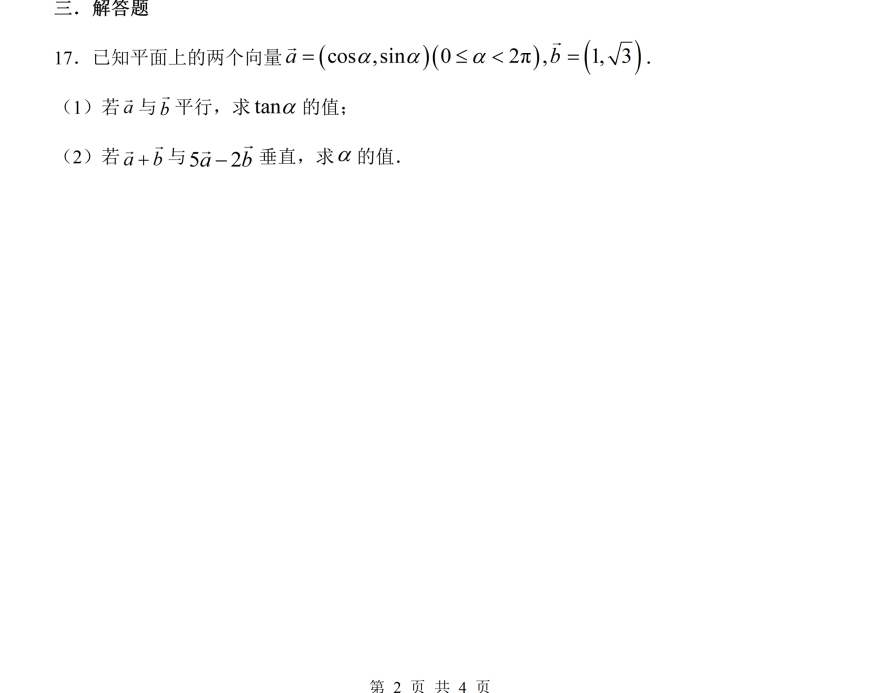
\includegraphics[width=0.96\linewidth]{crops/01-yziAF5kAbRtk3MMO-003-q17.png}
\caption{原图：\detokenize{documents/高一/01-yziAF5kAbRtk3MMO/003.png}}
\end{figure}
\vspace{0.4em}
\subsection*{5. 原卷第 7 题}
\textbf{来源}：【期末】上海市南洋模范中学2024-2025学年第二学期高一数学期末试卷

\begin{figure}[H]
\centering
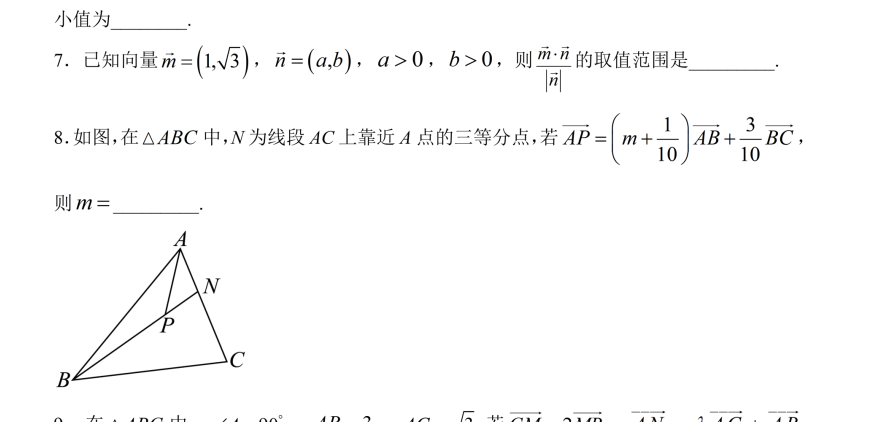
\includegraphics[width=0.96\linewidth]{crops/02-aF6bDvWUfZwct7Rz-002-q07.png}
\caption{原图：\detokenize{documents/高一/02-aF6bDvWUfZwct7Rz/002.png}}
\end{figure}
\vspace{0.4em}
\subsection*{6. 原卷第 12 题}
\textbf{来源}：【期末】上海市南洋模范中学2024-2025学年第二学期高一数学期末试卷

\begin{figure}[H]
\centering
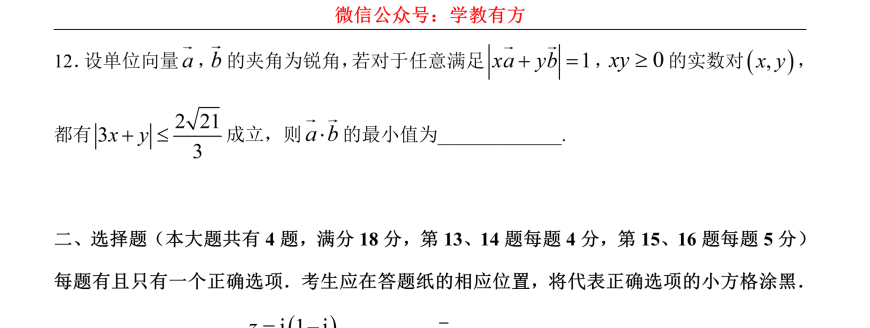
\includegraphics[width=0.96\linewidth]{crops/02-aF6bDvWUfZwct7Rz-003-q12.png}
\caption{原图：\detokenize{documents/高一/02-aF6bDvWUfZwct7Rz/003.png}}
\end{figure}
\vspace{0.4em}
\subsection*{7. 原卷第 17 题}
\textbf{来源}：【期末】上海市南洋模范中学2024-2025学年第二学期高一数学期末试卷

\begin{figure}[H]
\centering
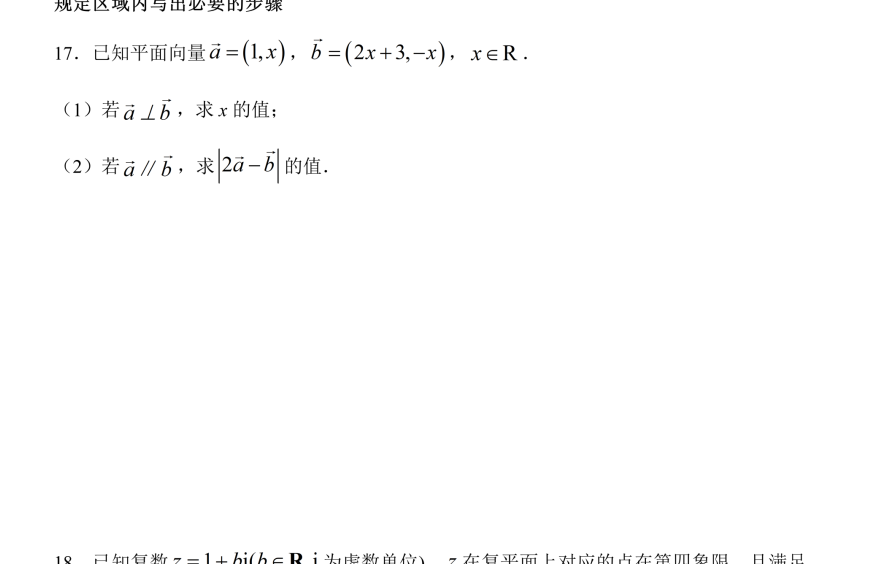
\includegraphics[width=0.96\linewidth]{crops/02-aF6bDvWUfZwct7Rz-004-q17.png}
\caption{原图：\detokenize{documents/高一/02-aF6bDvWUfZwct7Rz/004.png}}
\end{figure}
\vspace{0.4em}
\subsection*{8. 原卷第 20 题}
\textbf{来源}：【期末】上海市南洋模范中学2024-2025学年第二学期高一数学期末试卷

\begin{figure}[H]
\centering
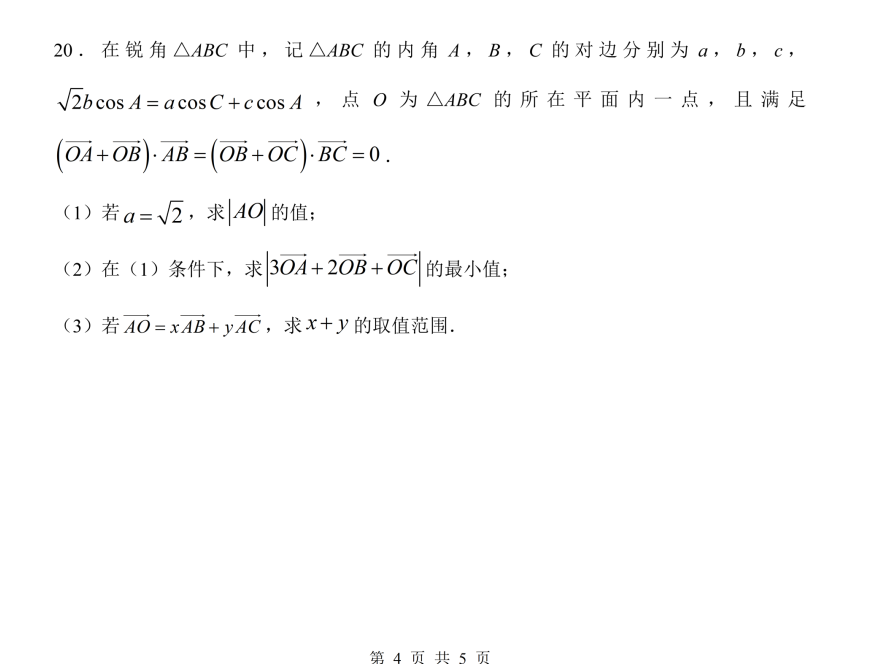
\includegraphics[width=0.96\linewidth]{crops/02-aF6bDvWUfZwct7Rz-005-q20.png}
\caption{原图：\detokenize{documents/高一/02-aF6bDvWUfZwct7Rz/005.png}}
\end{figure}
\vspace{0.4em}
\subsection*{9. 原卷第 3 题}
\textbf{来源}：【期末】上海市复兴中学2024-2025学年第二学期高一数学期末试卷

\begin{figure}[H]
\centering
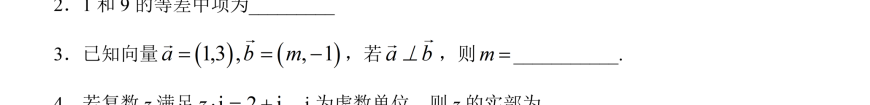
\includegraphics[width=0.96\linewidth]{crops/03-AeUS7-mBPoWmDxFx-002-q03.png}
\caption{原图：\detokenize{documents/高一/03-AeUS7-mBPoWmDxFx/002.png}}
\end{figure}
\vspace{0.4em}
\subsection*{10. 原卷第 6 题}
\textbf{来源}：【期末】上海市复兴中学2024-2025学年第二学期高一数学期末试卷

\begin{figure}[H]
\centering
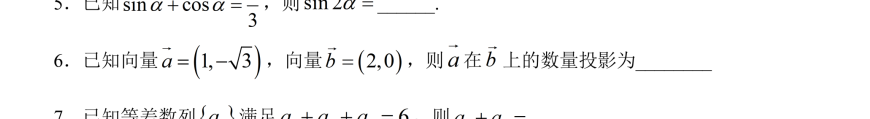
\includegraphics[width=0.96\linewidth]{crops/03-AeUS7-mBPoWmDxFx-002-q06.png}
\caption{原图：\detokenize{documents/高一/03-AeUS7-mBPoWmDxFx/002.png}}
\end{figure}
\vspace{0.4em}
\subsection*{11. 原卷第 11 题}
\textbf{来源}：【期末】上海市复兴中学2024-2025学年第二学期高一数学期末试卷

\begin{figure}[H]
\centering
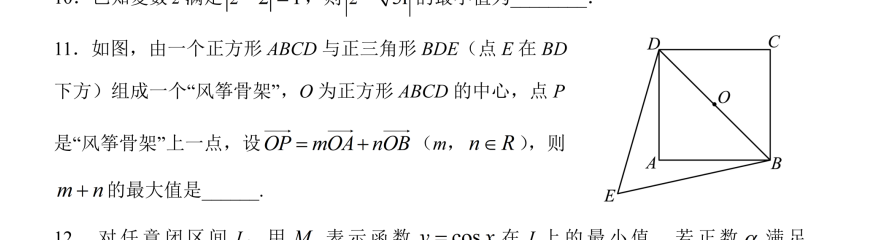
\includegraphics[width=0.96\linewidth]{crops/03-AeUS7-mBPoWmDxFx-002-q11.png}
\caption{原图：\detokenize{documents/高一/03-AeUS7-mBPoWmDxFx/002.png}}
\end{figure}
\vspace{0.4em}
\subsection*{12. 原卷第 19 题}
\textbf{来源}：【期末】上海市复兴中学2024-2025学年第二学期高一数学期末试卷

\begin{figure}[H]
\centering
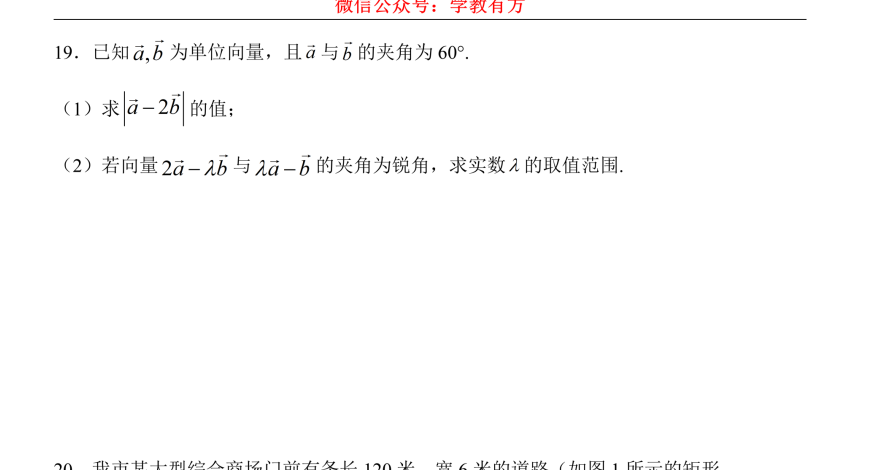
\includegraphics[width=0.96\linewidth]{crops/03-AeUS7-mBPoWmDxFx-004-q19.png}
\caption{原图：\detokenize{documents/高一/03-AeUS7-mBPoWmDxFx/004.png}}
\end{figure}
\vspace{0.4em}
\subsection*{13. 原卷第 21 题}
\textbf{来源}：【期末】上海市复兴中学2024-2025学年第二学期高一数学期末试卷

\begin{figure}[H]
\centering
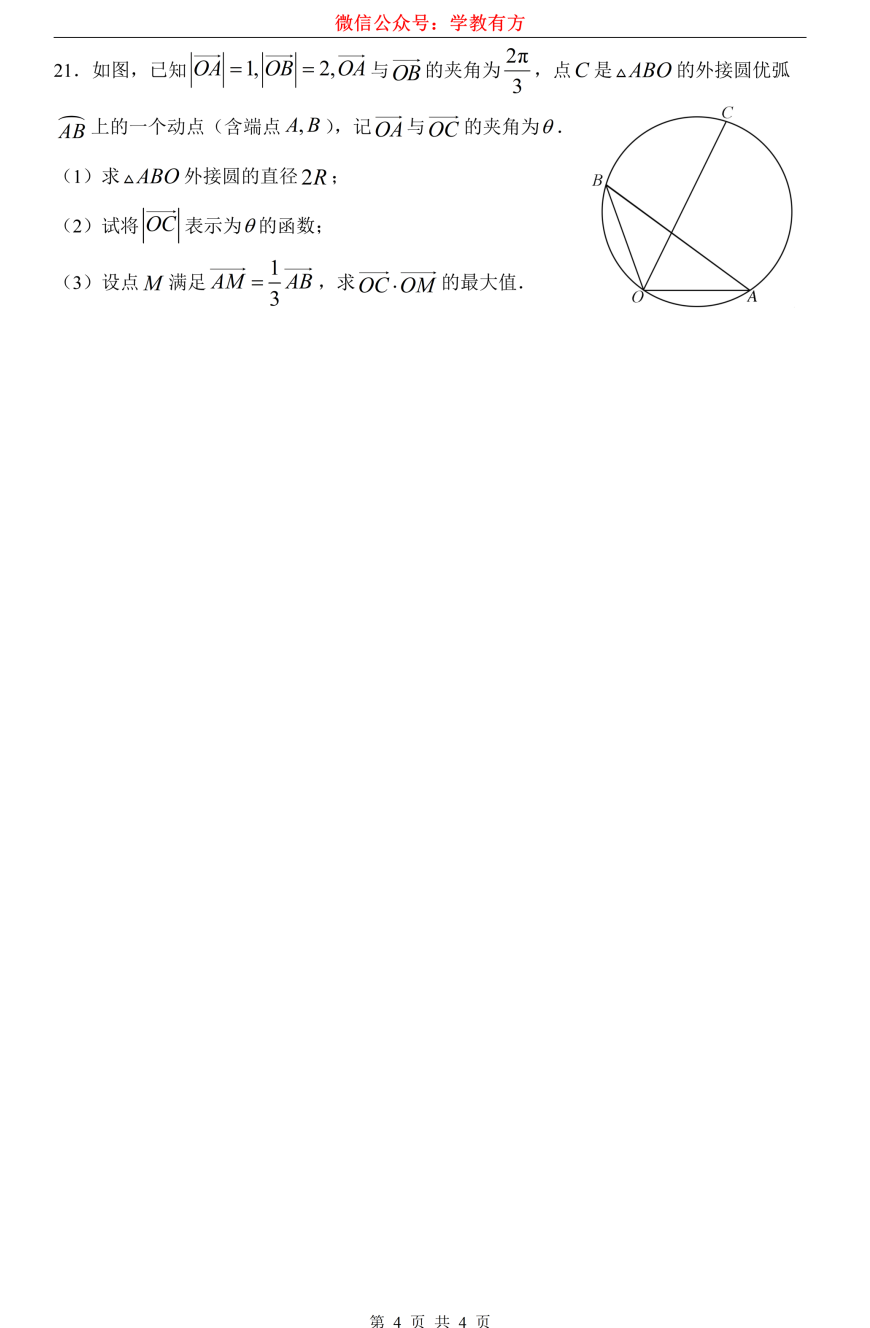
\includegraphics[width=0.96\linewidth]{crops/03-AeUS7-mBPoWmDxFx-005-q21.png}
\caption{原图：\detokenize{documents/高一/03-AeUS7-mBPoWmDxFx/005.png}}
\end{figure}
\vspace{0.4em}
\subsection*{14. 原卷第 6 题}
\textbf{来源}：【期末】上海市控江中学2024-2025学年第二学期高一数学期末试卷

\begin{figure}[H]
\centering
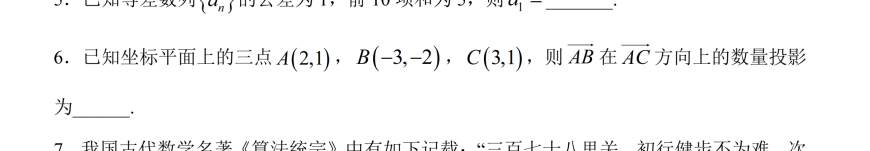
\includegraphics[width=0.96\linewidth]{crops/04-PspMJAQSNffj2NOH-002-q06.png}
\caption{原图：\detokenize{documents/高一/04-PspMJAQSNffj2NOH/002.png}}
\end{figure}
\vspace{0.4em}
\subsection*{15. 原卷第 12 题}
\textbf{来源}：【期末】上海市控江中学2024-2025学年第二学期高一数学期末试卷

\begin{figure}[H]
\centering
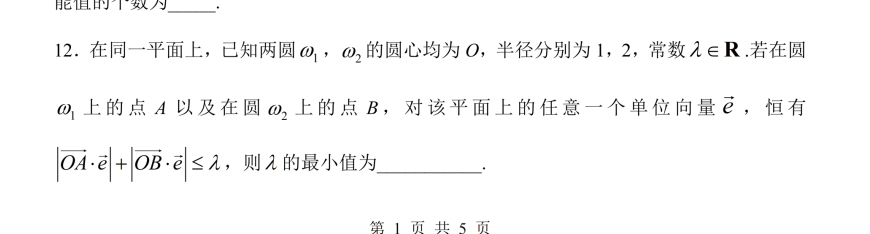
\includegraphics[width=0.96\linewidth]{crops/04-PspMJAQSNffj2NOH-002-q12.png}
\caption{原图：\detokenize{documents/高一/04-PspMJAQSNffj2NOH/002.png}}
\end{figure}
\vspace{0.4em}
\subsection*{16. 原卷第 20 题}
\textbf{来源}：【期末】上海市控江中学2024-2025学年第二学期高一数学期末试卷

\begin{figure}[H]
\centering
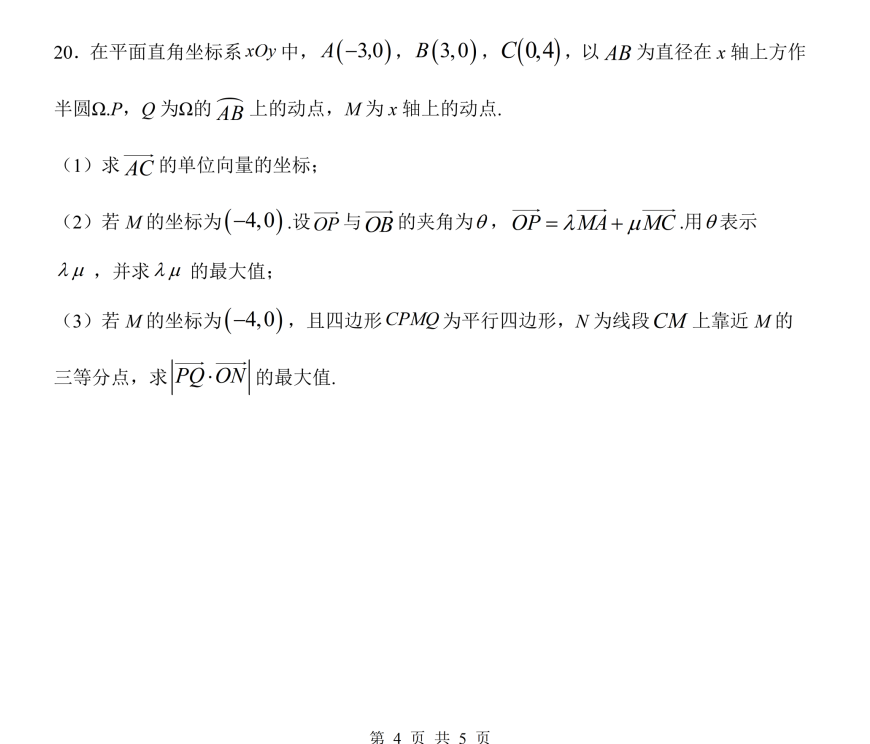
\includegraphics[width=0.96\linewidth]{crops/04-PspMJAQSNffj2NOH-005-q20.png}
\caption{原图：\detokenize{documents/高一/04-PspMJAQSNffj2NOH/005.png}}
\end{figure}
\vspace{0.4em}
\subsection*{17. 原卷第 5 题}
\textbf{来源}：【期末】上海市华东师范大学第二附属中学2024-2025学年第二学期高一数学期末试卷

\begin{figure}[H]
\centering
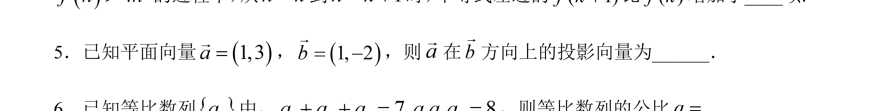
\includegraphics[width=0.96\linewidth]{crops/05-6PmxWuxmrPF6tcjf-002-q05.png}
\caption{原图：\detokenize{documents/高一/05-6PmxWuxmrPF6tcjf/002.png}}
\end{figure}
\vspace{0.4em}
\subsection*{18. 原卷第 11 题}
\textbf{来源}：【期末】上海市华东师范大学第二附属中学2024-2025学年第二学期高一数学期末试卷

\begin{figure}[H]
\centering
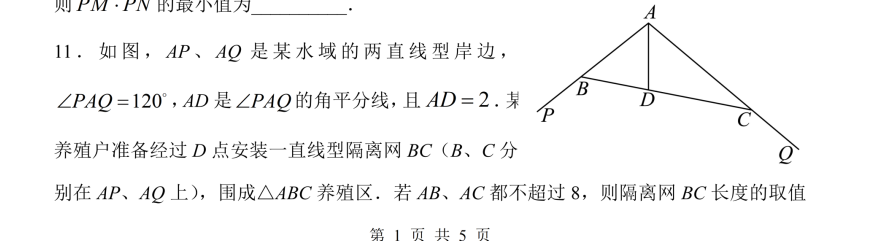
\includegraphics[width=0.96\linewidth]{crops/05-6PmxWuxmrPF6tcjf-002-q11.png}
\caption{原图：\detokenize{documents/高一/05-6PmxWuxmrPF6tcjf/002.png}}
\end{figure}
\vspace{0.4em}
\subsection*{19. 原卷第 17 题}
\textbf{来源}：【期末】上海交通大学附属中学2024-2025学年第二学期高一数学期末试卷

\begin{figure}[H]
\centering
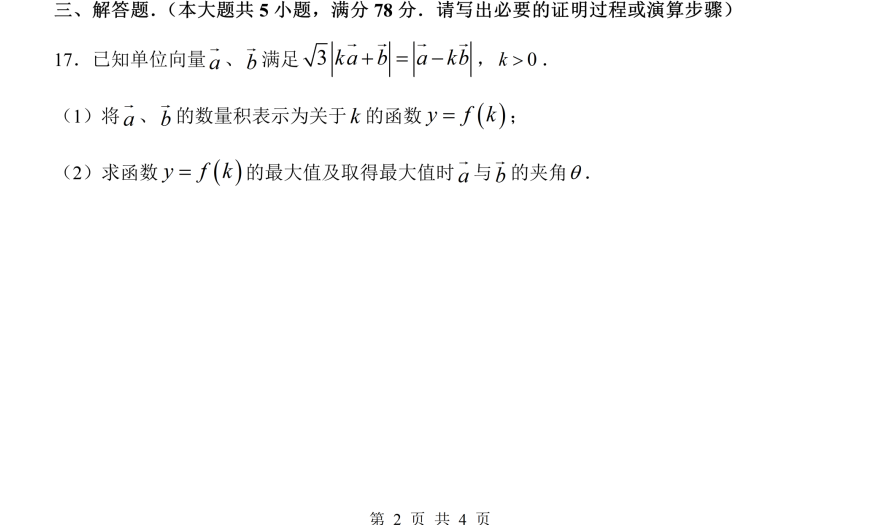
\includegraphics[width=0.96\linewidth]{crops/06-4EnOr70jpgX8ucy5-003-q17.png}
\caption{原图：\detokenize{documents/高一/06-4EnOr70jpgX8ucy5/003.png}}
\end{figure}
\vspace{0.4em}
\subsection*{20. 原卷第 19 题}
\textbf{来源}：【期末】上海交通大学附属中学2024-2025学年第二学期高一数学期末试卷

\begin{figure}[H]
\centering
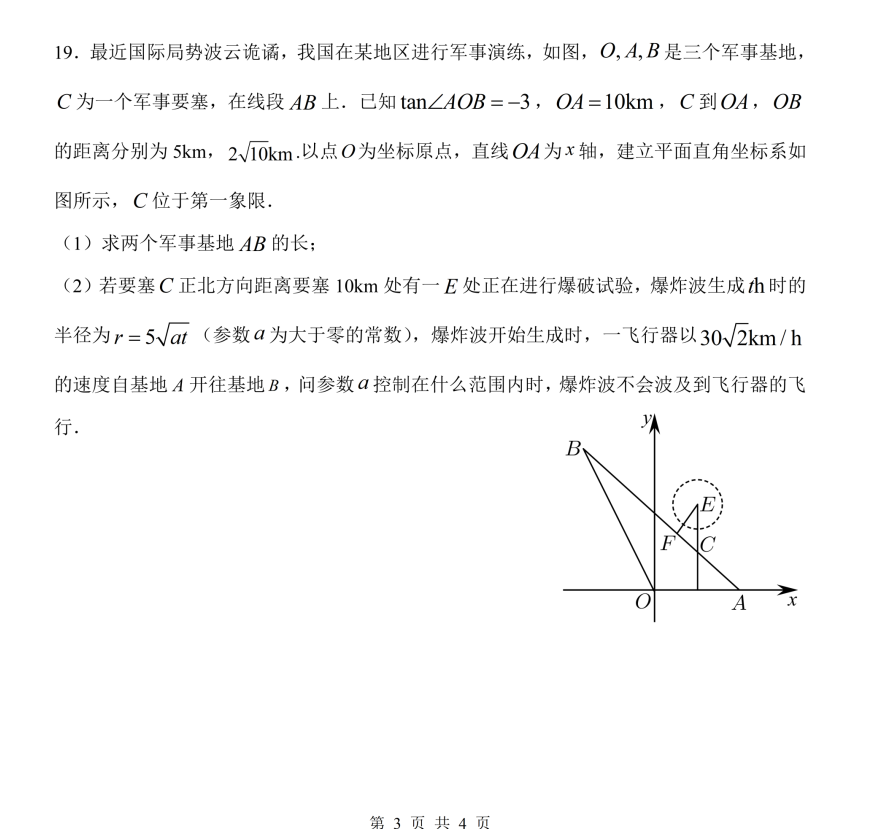
\includegraphics[width=0.96\linewidth]{crops/06-4EnOr70jpgX8ucy5-004-q19.png}
\caption{原图：\detokenize{documents/高一/06-4EnOr70jpgX8ucy5/004.png}}
\end{figure}
\vspace{0.4em}
\subsection*{21. 原卷第 6 题}
\textbf{来源}：【期末】上海市复旦大学附属中学2024-2025学年第二学期高一数学期末试卷（B）

\begin{figure}[H]
\centering
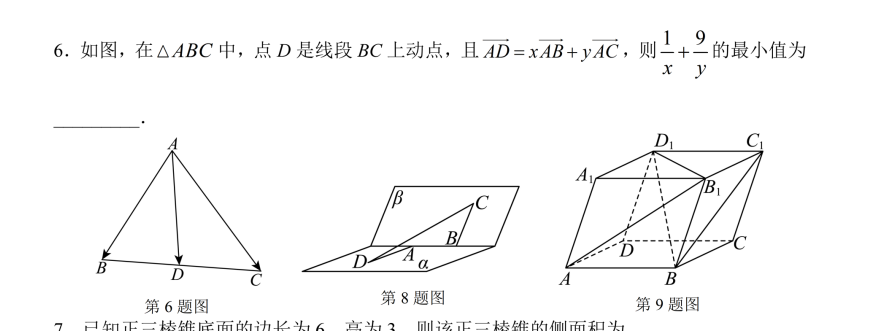
\includegraphics[width=0.96\linewidth]{crops/07-lXolUr-1bu6QRhI1-002-q06.png}
\caption{原图：\detokenize{documents/高一/07-lXolUr-1bu6QRhI1/002.png}}
\end{figure}
\vspace{0.4em}
\subsection*{22. 原卷第 17 题}
\textbf{来源}：【期末】上海市复旦大学附属中学2024-2025学年第二学期高一数学期末试卷（B）

\begin{figure}[H]
\centering
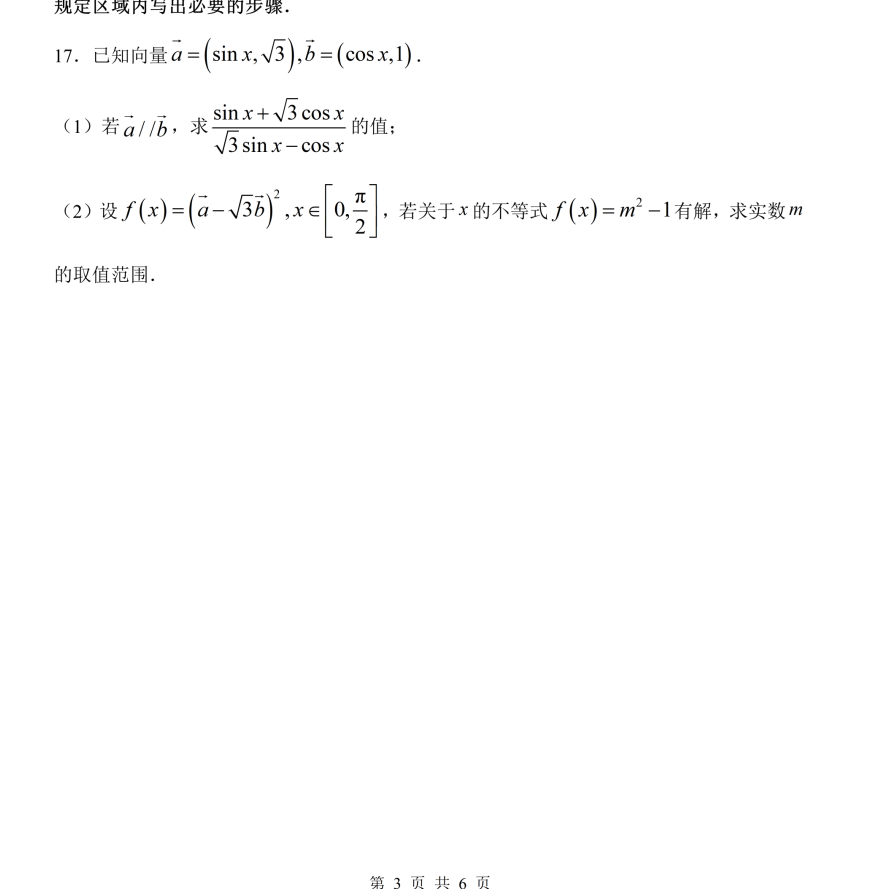
\includegraphics[width=0.96\linewidth]{crops/07-lXolUr-1bu6QRhI1-004-q17.png}
\caption{原图：\detokenize{documents/高一/07-lXolUr-1bu6QRhI1/004.png}}
\end{figure}
\vspace{0.4em}
\subsection*{23. 原卷第 20 题}
\textbf{来源}：【期末】上海市复旦大学附属中学2024-2025学年第二学期高一数学期末试卷（B）

\begin{figure}[H]
\centering
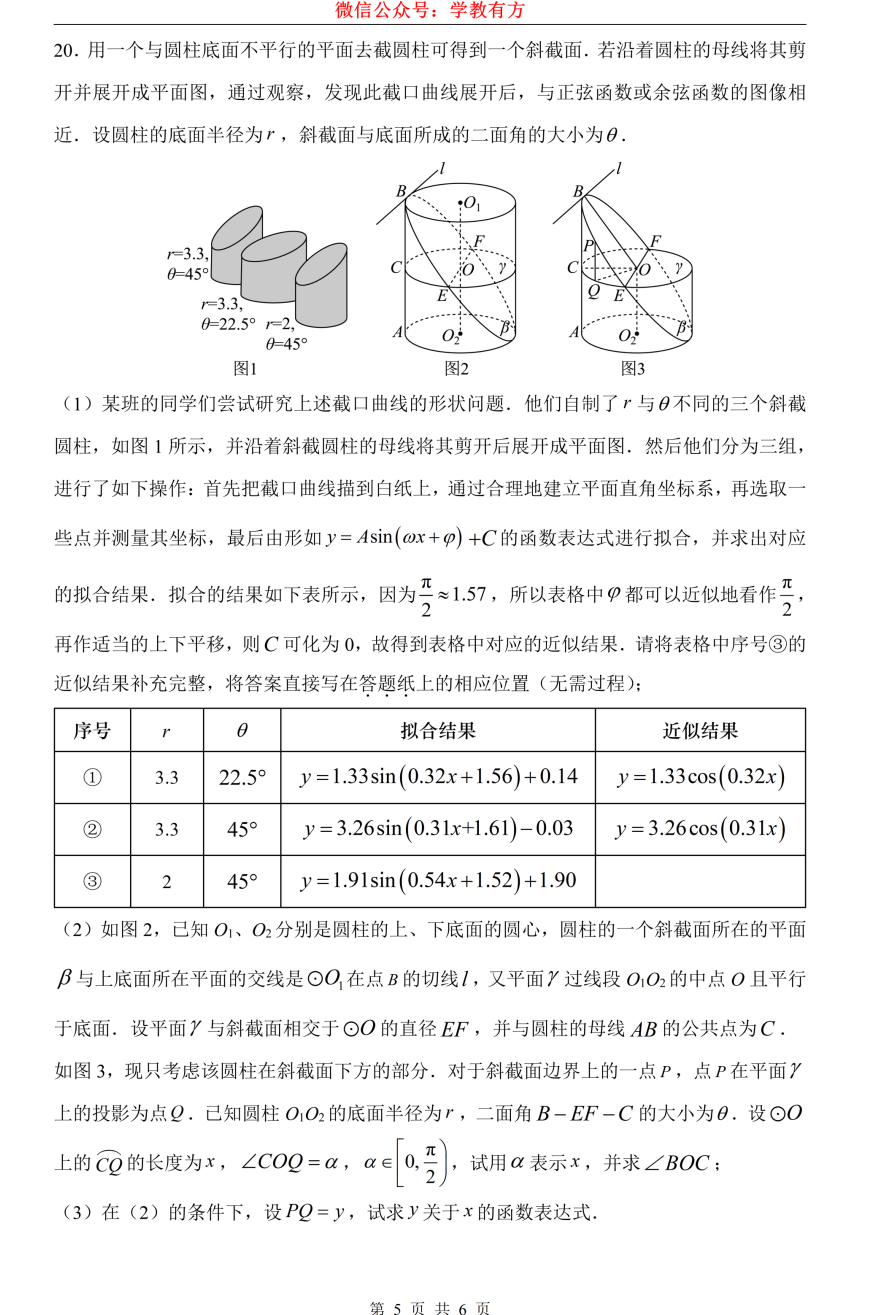
\includegraphics[width=0.96\linewidth]{crops/07-lXolUr-1bu6QRhI1-006-q20.png}
\caption{原图：\detokenize{documents/高一/07-lXolUr-1bu6QRhI1/006.png}}
\end{figure}
\vspace{0.4em}
\end{document}
